\documentclass{matmex-diploma-custom}
\usepackage{listings}  
\usepackage{hyperref}
\usepackage{verbments}
\usepackage{minted}
\usepackage{caption}
\usepackage{fancybox}
\newfontfamily{\cyrillicfonttt}{CMU Serif}

\lstset{
basicstyle=\small,
identifierstyle=\ttfamily,
keywordstyle=\bfseries,
commentstyle=\scriptsize\rmfamily,
basewidth={0.5em,0.5em},
fontadjust=true,
escapechar=~,
language=haskell
}
\begin{document}
% Год, город, название университета и факультета предопределены,
% но можно и поменять.
% Если англоязычная титульная страница не нужна, то ее можно просто удалить.
\filltitle{ru}{
    chair              = {Кафедра Системного Программирования},
    title              = {Декларативное форматирование в режиме онлайн},
    % Здесь указывается тип работы. Возможные значения:
    %   coursework - Курсовая работа
    %   diploma - Диплом специалиста
    %   master - Диплом магистра
    %   bachelor - Диплом бакалавра
    type               = {coursework},
    position           = {студента},
    group              = 344,
    author             = {Озерных Игорь Станиславович},
    supervisorPosition = {асп.},
    supervisor         = {Подкопаев А.\,В.},
    reviewerPosition   = {ст. преп.},
    reviewer           = {--},
    chairHeadPosition  = {д.\,ф.-м.\,н., профессор},
    chairHead          = {Терехов А.\,Н.},
%   university         = {Санкт-Петербургский Государственный Университет},
%   faculty            = {Математико-механический факультет},
%   city               = {Санкт-Петербург},
%   year               = {2015}
}

\maketitle
\tableofcontents

\section*{Введение}

Ручное управление памятью в языках, подобных C++, является источником большого количества трудно отслеживаемых ошибок, наличия которых можно было бы
избежать, сделав процесс управления памятью автоматическим. \textit{Сборка мусора} является одним из способов автоматического управления памятью, при
котором освобождение памяти выводится из-под контроля ПО на прикладном уровне. При автоматическом управлении программист не может явно влиять на распределение
объектов в памяти, у него есть лишь
косвенные способы сделать это с помощью использования тех или иных языковых конструкций. В идеальном случае, для рационального использования
памяти необходимо освобождать память, занимаемую объектами, которые более не будут использованы программой. Поскольку точно определить, что
объект не будет использован в дальнейшем, невозможно, на практике используют критерий доступности. \textit{Доступность} --- это консервативное
приближение используемости. \textit{Мусором}, в таком случае, называют объект, все пути доступа к которому уже разрушены, а память из-под него
ещё не освобождена. В некоторое, заранее определенное время, например, в простейшем случае, когда перестаёт хватать свободной памяти, выполнение
программы временно приостанавливается и запускается процесс \textit{сборки мусора}, который освобождает всю или ту, что возможно, память,
занятую мусором, после чего управление возвращается обратно программе. \textit{Сборщиком мусора} называется компонент, производящий \textit{сборку мусора}.

Процесс \textit{сборки мусора}, в простейшем случае, делят на три этапа:
\begin{enumerate}
\item \textit{Построение корневого множества}. На этом этапе строится множество объектов, которые считаются изначально доступными.
Такие объекты называются \textit{корнями} (англ. roots). Данное построение
аксиоматично, т.е. основывается на некотором наборе правил, согласно которым те или иные элементы считаются доступными. Данный этап является неотъемлемой
частью любого сборщика мусора.
\item \textit{Маркировка}. Начиная с множества, построенного на предыдущем этапе, происходит сканирование памяти, и все объекты, до которых возможно
добраться из построенного корневого множества, считаются доступными; оставшиеся объекты считаются мусором.
\item \textit{Освобождение}. Происходит сканирование кучи, в течение которого память из-под всех элементов, помеченных как мусор или не отмеченных как
доступные, освобождается.
\end{enumerate}

Есть несколько требований, которые должны быть выполнены для реализации сборки мусора:
\begin{enumerate}
\item Возможность построения корневого множества. Иными словами, необходимо иметь возможность идентифицировать все указатели в программном стеке, регистрах
и статической области памяти.
\item Должна присутствовать возможность определить все указатели из любого объекта на другие элементы кучи.
\end{enumerate}
В таких языках, как LISP или JAVA все условия соблюдаются, и в них успешно используется технология сборки мусора, в то время как, например,
в языке C не все условия выполняются. В языках, где не соблюдаются хотя бы одно из вышеперечисленных условий, возможна исключительна
\textit{консервативная сборка мусора}.
\textit{Консервативной} называется такая сборка мусора, при которой любой элемент данных, значение которого может быть истолковано, как указатель на
некоторый элемент кучи, считается  таковым. Консервативный подход к сборке мусора не позволяет собрать весь мусор, что может стать проблемой при обработке
большого количества данных. Неконсервативная сборка мусора лишена подобного недостатка и способна освободить всю память программы, более не
являющуюся доступной. \textit{Неконсервативным} или  \textit{точным сборком мусора} называется сборщик мусора, имеющий возможность точно распознать
все указатели в памяти. Иными словами, точный сборщик мусора --- это сборщик мусора, не использующий консервативный подход.

В C++ не соблюдаются требования, необходимые для сборки сборки мусора, реализовать точный сборщик мусора без ограничений
на использование некоторых примитивов языка не представляется возможным.
Более того, в C++ имеется ряд технических сложностей, затрудняющих реализацию точного сборщика мусора.
Тем не менее, в случае соблюдения программистом некоторых соглашений на програмный код,
точная сборка мусора становится возможной и в C++.

Целями работы является реализация основных примитивов библиотеки неконсервативной сборки мусора для C++,
обеспечение возможности совмещения ручного и автоматического управления памятью.
\newpage
\section{Обзор существующих библиотек}

В рамках исследования был проведен анализ основных существующих функциональных принтер-библиотек. Все выбранные библиотеки оказались комбинаторными, что естественно для функциональных языков.

% Так как работа проводилась в контексте функциональных языков, для анализа были выбраны комбинаторные библиотеки.
% Комбинаторы естественным образом возникают при наличии в языке функций высших порядков.

\subsection{Модельный язык L}
% \addcontentsline{toc}{section}{Модельный язык L}

В дальнейшем центральным примером, для которого мы будем разрабатывать принтеры, будет модельный язык L. Именно для этого языка будет реализован шаблонный принтер.

Язык L состоит из небольшого числа операторов:
\begin{enumerate}
	\item присваивание;
	\item цикл с предусловием;
	\item ветвление;
	\item последовательное выполнение;
	\item чтение с занесением в переменную;
	\item печать целочисленного выражения.
\end{enumerate}

Также в языке есть выражения. Выражения бывают трех типов:
\begin{enumerate}
	\item константа;
	\item переменная;
	\item бинарная операция.
\end{enumerate}

На рисунке~\ref{fig:lEx} приведен пример программы на языке L. В данном случае, это программа, которая считывает с консоли два числа, а потом возводит второе число в степень, равную первому.

\begin{figure}[h!]
	\centering
	% \inputminted{pascal}{codes/lEx.l}
	\lstinputlisting[language=llang]{codes/lEx.l}
	\caption{Быстрое возведение в степень на языке L}
	\label{fig:lEx}
\end{figure}

\subsection{Библиотека Хьюза}

Библиотека Джона Хьюза\cite{hughes} считается первой комбинаторной принтер-библиотекой. Она основана на алгоритме, предложенном Дереком Оппеном \cite{oppen}, и по сути является его реализацией в функциональном стиле на языке Haskell\footnote{http://haskell.org}. Также библиотека Хьюза, расширенная Саймоном Пейтоном Джонсом \cite{peytonJones}, является стандартной принтер-библиотекой для языка Haskell.

% рассказать об оптимальном

В данной библиотеке ключевым типом является “\lstinline[language=Haskell]{Doc}”. Он представляет документ, который потом может быть переведен в строковое представление.
Основные комбинаторы для составления документа:
% \inputminted{haskell}{Podkopaev/codes/hughesBasicOperators.hs}
\lstinputlisting[language=Haskell]{Podkopaev/codes/hughesBasicOperators.hs}

Так, с помощью функции “\lstinline[language=Haskell]{text}” по строке получается документ, оператор “\textbf{<>}” соединяет два документа горизонтально (см. рисунок~\ref{fig:hughesHorComp}), а оператор “\textbf{\$\$}” соединяет документы вертикально (см. рисунок~\ref{fig:hughesVertComp}).

\begin{figure}[ht]
	\begin{subfigure}[b]{0.45\linewidth}
		\centering
		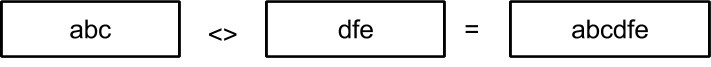
\includegraphics[width=\textwidth]{hughesHorComp}
		\caption{Комбинатор “\textbf{<>}”}
		\label{fig:hughesHorComp}
	\end{subfigure}
	\hspace{0.5cm}
	\begin{subfigure}[b]{0.45\linewidth}
		\centering
		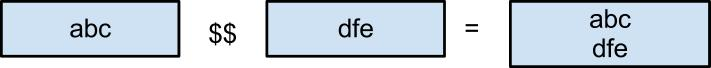
\includegraphics[width=\textwidth]{hughesVertComp}
		\caption{Комбинатор “\textbf{\$\$}”}
		\label{fig:hughesVertComp}
	\end{subfigure}

	\caption{Пример работы комбинаторов}
\end{figure}

Функция “\lstinline[language=Haskell]{nest}” добавляет к каждой строке документа заданное число ведущих пробелов. Функция “\lstinline[language=Haskell]{sep}” является ключевым комбинатором, который в этой библиотеке позволяет задавать плавающую раскладку документа. Она принимает как параметр список документов, а на выходе получается документ, который представляет из себя либо вертикальную склейку элементов списка, либо горизонтальную склейку (в этом случае если к документу из списка применялась функция “\lstinline[language=Haskell]{nest}”, то к этому документу не добавляются ведущие пробелы, то есть применение “\lstinline[language=Haskell]{nest}” попросту игнорируется), причем между документами вставляется пробельный символ. Вариант раскладки выбирается функцией “\lstinline[language=Haskell]{pretty}”:

% \inputminted{haskell}{Podkopaev/codes/hughesPretty.hs}
\lstinputlisting[language=Haskell]{Podkopaev/codes/hughesPretty.hs}

Кроме самого документа, функция “\lstinline[language=Haskell]{pretty}” также принимает два числа: максимальную длину и максимальную наполненность строки. Здесь наполненность строки значит длину текста без ведущих пробельных символов. В ходе работы этой функции и происходит выбор раскладки документа, полученного с помощью комбинатора “\lstinline[language=Haskell]{sep}”. Если горизонтальная раскладка удовлетворяет ограничениям на ширину строки, то она и выбирается. Иначе выбирается вертикальная раскладка.


% Возможно, стоит сделать после обзора всех библиотек

Рассмотрим пример описания принтера с помощью библиотеки Хьюза. Для этого используем учебный язык L. Часть принтера для языка L, отвечающая за представление операторов, показана на рисунке~\ref{fig:lHughesPrinter}.
В примере используется не описанный выше комбинатор “\lstinline[language=Haskell]{<+>}”, который определяется следующим образом:

\lstinputlisting[language=Haskell]{Podkopaev/codes/hughesAddComb.hs}

\begin{figure}[h!]
	% \inputminted{haskell}{Podkopaev/codes/lHughesPrinter.hs}
	\lstinputlisting[language=Haskell]{Podkopaev/codes/lHughesPrinter.hs}
	\caption{Принтер, написанный с помощью библиотеки Хьюза}
	\label{fig:lHughesPrinter}
\end{figure}

В данном случае принтер получился несложным, но абсолютно не наглядным. Поскольку в библиотеке нет механизмов, позволяющих явно варьировать раскладку документа в зависимости от раскладки его поддокументов, невозможно выразить пример с рисунка~\ref{fig:lGoodWriteEx}.
То есть, в случае многострочного выражения в операторе “\lstinline[language=llang]{write}”, напечатать закрывающую скобку на уровне самого оператора.

\begin{figure}[h!]
	% \inputminted{pascal}{Podkopaev/codes/lGoodWriteEx.l}
	\lstinputlisting[language=llang]{Podkopaev/codes/lGoodWriteEx.l}
	\caption{Желательный пример печати конструкции “\lstinline[language=llang]{write}”}
	\label{fig:lGoodWriteEx}
\end{figure}

С помощью реализации принтера с рисунка~\ref{fig:lHughesPrinter}, в данном случае для оператора “\lstinline[language=llang]{write}” получится немного не то (см. рисунок~\ref{fig:lCurWriteEx}).
\begin{figure}[h!]
	% \inputminted{pascal}{Podkopaev/codes/lCurWriteEx.l}
	\lstinputlisting[language=llang]{Podkopaev/codes/lCurWriteEx.l}
	\caption{Результат для изначального принтера конструкции “\lstinline[language=llang]{write}”}
	\label{fig:lCurWriteEx}
\end{figure}

Если попробовать поменять функцию “\lstinline[language=Haskell]{docFromOperation}” для конструкции “\lstinline[language=llang]{write}” (см. рис. \ref{fig:lHughesWriteChange}),
то для многострочного выражения все получится правильно, но в случае однострочного --- появится лишний пробел перед закрывающей скобкой (см. рис. \ref{fig:lBadWriteEx})).

\begin{figure}[h!]
	% \inputminted{haskell}{Podkopaev/codes/lHughesWriteChange.hs}
	\lstinputlisting[language=Haskell]{Podkopaev/codes/lHughesWriteChange.hs}
	\caption{Измененный принтер конструкции “\lstinline[language=llang]{write}”}
	\label{fig:lHughesWriteChange}
\end{figure}

\begin{figure}[h!]
	% \inputminted{pascal}{Podkopaev/codes/lBadWriteEx.l}
	\lstinputlisting[language=llang]{Podkopaev/codes/lBadWriteEx.l}
	\caption{Результат для измененого принтера конструкции “\lstinline[language=llang]{write}”}
	\label{fig:lBadWriteEx}
\end{figure}
\newpage

\subsection{Принтер-комбинаторная библиотека Вадлера}

В \cite{wadler} Филипп Вадлер описал свою комбинаторную бибилиотеку для форматированного вывода на языке Haskell. Она является модификацией библиотеки Хьюза, описанной в предыдущем разделе. Код библиотеки сократился с $\approx$ 110 строк до $\approx$ 80 строк, и, по исследованию Вадлера, на 30\% увеличилась скорость вычисления раскладки документа.

Рассмотрим основые комбинаторы этой библиотеки:
% \inputminted{haskell}{codes/wadlerBasicOperations.hs}
\lstinputlisting[language=Haskell]{codes/wadlerBasicOperations.hs}

Вадлер решил отказаться от двух разных способов соединения документов, оставив лишь горизонтальную склейку. Но для того, чтобы можно было выражать не только однострочные документы, в библиотеке Вадлера появилась функция “\lstinline[language=Haskell]{line}”. Она создает документ, который может быть переведен в символ новой строки или в пробел.
Функция “\lstinline[language=Haskell]{group}” имеет то же назначение, что и оператор “\lstinline[language=Haskell]{sep}” в библиотеке Хьюза, но работает не со списком документов, а с одним документом, и по сути предоставляет альтернативы для алгоритма перевода документа в “\lstinline[language=Haskell]{String}”: в документе, на который подействовал “\lstinline[language=Haskell]{group}”, либо все вхождения “\lstinline[language=Haskell]{line}” заменяются на пробел, либо остаются переводами строки (если они не являются частью вложенных “\lstinline[language=Haskell]{group}”-документов).

В таком виде библиотека потеряла в выразительности, что признается в статье Вадлера. Но кроме потери выразительности, есть еще один серьезный недостаток, возникающий из-за оператора “\lstinline[language=Haskell]{group}”. То, что любой документ им может быть преобразован в однострочный, делает библиотеку неприменимой в некоторых ситуациях. 

Рассмотрим следующий пример. Пусть нам надо написать принтер для языка Python\footnote{http://python.org}. Для конструкции последовательных операторов принтер изображен на рисунке~\ref{fig:pythonPrinter}.
По-другому его написать нельзя --- мы хотим, чтобы последовательные операторы печатались на новых строках. Но если такая конструкция попадет внутрь “\lstinline[language=Haskell]{group}”-документа, то последовательные строчки могут склеиться пробелом, что сделает код некорректным, так как в Python несколько операторов на одной строке должны разделяться символом “;”.

\begin{figure}[h!]
	% \inputminted{haskell}{codes/pythonPrinter.hs}
	\lstinputlisting[language=Haskell]{codes/pythonPrinter.hs}
	\caption{Принтер для последовательных операторов в Python}
	\label{fig:pythonPrinter}
\end{figure}

Так корректный код (см. рисунок~\ref{fig:pythonCode}) может превратиться в некорректный (см. рисунок~\ref{fig:pythonCodeBad}).
\begin{figure}[h!]
	\centering
	\null\hfill
	\subfloat[]{
		\centering
		\lstinputlisting[language=Python]{codes/pythonCode.py}
		\label{fig:pythonCode}	
	}
	\null\hfill
	\subfloat[]{
		\centering
		\lstinputlisting[language=Python]{codes/pythonCodeBad.py}
		\label{fig:pythonCodeBad}
	}
	\hfill
	\null
	\caption{Пример работы принтера для языка Python}
\end{figure}

\newpage

\subsection{Библиотека Азеро и Свиерстры}

Библиотека Азеро и Свиерстры\footnote{
В данном тексте, с целью не усложнять восприятие, изменены обозначения комбинаторов библиотеки Свиерстры на обозначения, подобные тем, что были уже рассмотрены в библиотеке Хьюза. Семантика комбинаторов описана без изменений, согласно оригинальной статье и соответствующей библиотеке.
}, описанная в \cite{swierstra}, отличается от предыдущих библиотек тем, что дает возможность явным образом задать несколько несвязанных вариантов раскладки документа. В этой библиотеке есть комбинатор “\lstinline[language=Haskell]{<|>}”:

% \inputminted{haskell}{Podkopaev/codes/chooseSw.hs}
\lstinputlisting[language=Haskell]{Podkopaev/codes/chooseSw.hs}

Этот комбинатор берет два документа и создает новый, который при раскладке может стать первым или вторым, в зависимости от того, какой из документов раскладывается оптимальней. \textit{Оптимальной} раскладкой для документа считается раскладка, удовлетворяющая ограничению на ширину документа и имеющая минимальную высоту.

Наличие комбинатора “\lstinline[language=Haskell]{<|>}” сразу же решает проблему со скобкой, которая была поднята в обзоре библиотеки Хьюза (см. рис.~\ref{fig:bracketSwierstra}).\footnote{
	В примере используется функция “\lstinline[language=Haskell]{element_h1}”. Эта функция выбирает из вариантов раскладки документа те, которые имеют высоту 1.
}

\begin{figure}[h!]
	% \inputminted{haskell}{Podkopaev/codes/bracketSwierstra.hs}
	\lstinputlisting[language=Haskell]{Podkopaev/codes/bracketSwierstra.hs}
	\caption{Принтер конструкции “\lstinline{write}”, удовлетворяющий примеру с рис.~\ref{fig:lGoodWriteEx}}
	\label{fig:bracketSwierstra}
\end{figure}

% Данная вариативность достигается за счет особого представления документа. В данной библиотеке он представляется как ленивый список раскладок, причем список отсортирован в порядке возрастания количества строк раскладки.

Библиотека Азеро и Свиерстры обладает самым богатым набором комбинаторов и, благодаря оператору “\lstinline[language=Haskell]{<|>}”, позволяет выразить практически любые принтеры. Но, также как остальные рассмотренные библиотеки, не дает механизмов для простого и наглядного задания принтеров.
\newpage
\section{Реализация}

Контекстом данной работы является разработка метода задания принтеров с помощью шаблонов.
Под \emph{шаблоном} здесь и далее понимаются данные, сопоставляя которые с
переданным на печать синтаксическим деревом, мы будем получать текстовое представление
для этого дерева. Более точно, каждый конкретный шаблон позволяет построить
текстовые представления для подходящего по типу 
узла синтаксического дерева, используя уже полученные представления дочерних поддеревьев.

Фактически в реализации шаблон --- это размеченное дерево разбора
некоторой синтаксической конструкции, в котором по каждой метке можно выяснить
ограничения на представление соответствующих поддеревьев и описание, каким
образом нужная раскладка поддерева должна быть вставлена в шаблон.
При этом сами шаблоны получаются из некоторого эталонного репозитория с исходном
кодом на целевом языке определяемого принтера.
Так, к примеру, принтер будет использовать форматирование GNU, если ему на вход
передать один или несколько проектов в СК GNU.

Кроме того, полученный таким образом принтер должен выдавать оптимальное представление
для синтаксического дерева, переданного на печать. На нижнем уровне в принтере 
используются оптимальные принтер-комбинаторы с выбором. Здесь комбинатор выбора нужен
для возможности задания вариантов представления, соответствующих разным шаблонам.
Недостатком существующих оптимальных принтер-комбинаторов с выбором \cite{swierstra}
является их экспоненциальная сложность. Поэтому для возможности использования того же
комбинаторного интерфейса в рамках данной работы с помощью BURS была разработана
полиномиальная версия этих комбинаторов~\cite{podkopaevBoulytchev}.

Для апробации метода в случае языка Java был разработан принтер-плагин для
IntelliJ IDEA, что позволило переиспользовать синтаксический анализатор Java
для получения шаблонов.
Разработка велась на языке Kotlin.
Kotlin\footnote{\cd{http://kotlin.jetbrains.org/}}
--- это функциональный, объектно-ориентированный, компилируемый
в JVM-байткод и JavaScript язык, разрабатываемый компанией
JetBrains\footnote{\cd{http://jetbrains.org/}}.
Kotlin был выбран для реализации принтер-плагина к IntelliJ IDEA по нескольким
причинам. 
Во-первых, Kotlin обладает хорошей интеграцией с Java, что позволяет
использовать его с IDEA API. 
Во-вторых, функции в Kotlin являются объектами первого рода, что позволяет
легко реализовывать комбинаторные библиотеки на нем.
На данный момент Kotlin находится в стадии разработки, поэтому
периодически возникают
проблемы с тем, что исходные коды перестают быть совместимыми с новыми
версиями языка,
но обычно требуется внести небольшой набор исправлений для
восстановления работоспособности.

% \subsection{Полиномиальной сложности принтер-комбинаторы с выбором}

\subsection{Оптимальное форматирование как задача BURS}

Для снижения алгоритмической сложности задачи поиска
оптимального представления документа, заданного комбинаторами из \cite{swierstra},
можно произвести сведение к BURS.
Сведение основано на следующих наблюдениях.
Пусть $w$ есть максимальная допустимая
ширина вывода. Поскольку каждая возникающая раскладка представляется блоком
текста, для поиска оптимального представления можно рассматривать
все промежуточные раскладки
как тройки $(n, k, h)$, где $n \le w$ --- это общая ширина раскладки, $k \le n$ ---
ширина ее последней строчки, $h$ --- ее высота. Тогда очевидно, что при $h_1 \le h_2$
между $(n, k, h_1)$ и $(n, k, h_2)$ первая тройка предпочтительней на любом этапе вычислений.
Таким образом для каждого узла не может быть более $w^2$ существенных представлений\footnote{
На самом деле, из-за ограничения $k \le n$ максимальное число раскладок не $w^2$, a
$\frac{w^2 + w}{2}$, но это несущественно.}.

Документ, для которого мы ищем раскладку, можно рассматривать как дерево, построенное из примитивов
\lstinline[language=Haskell]{text},
\lstinline[language=Haskell]{indent},
\lstinline[language=Haskell]{beside},
\lstinline[language=Haskell]{above} и \lstinline[language=Haskell]{choice}. Тогда задачу
раскладки документа можно решать независимо для поддеревьев, а потом объединять решения
при учете, что для каждого поддерева
и каждой пары $(n, k), k \le n \le w$ запоминается такая минимальная $h$, что для поддерева существует
текстовое представление с размерами $(n, k, h)$. Тогда, совершив обход дерева снизу вверх, мы сможем
вычислить оптимальное представление для всего дерева. Полезно заметить,
что оптимальное представление дерева не всегда получается из оптимальных представлений его
поддеревьев, поскольку при использовании поддеревьев возникают дополнительные
ограничения на ширину раскладок этих поддеревьев.

Приведенные наблюдения можно формализовать в виде BURS-задачи.
Для заданной ширины вывода $w$ введем набор нетерминалов
$T_n^k$, для всех $k \le n \le w$. Определим BURS-грамматику так, чтобы цена вывода $h$ нетерминала
$T_n^k$ для документа соответствовала его раскладке с параметрами $(n, k, h)$.
Для такой BURS-грамматики этап разметки посчитает все существенные раскладки, а этап свертки
вернет оптимальную. Определим правила переписывания для этой грамматики:
\begin{enumerate}
\item Для терминального узла $[\mbox{\lstinline{text s}}]$\footnote{
  Квадратные скобки используются для обозначения терминалов, состоящих из одного
  или нескольких символов.}
  существует два варианта:
  \begin{itemize}
     \item Если $|s|\le w$ (где $|s|$ --- это длина строки $s$), то вводится единственное правило
           $T^{|s|}_{|s|}: [\mbox{\lstinline{text s}}]$ со стоимостью $1$;           
           для всех остальных
           $k, n\ne |s|$ используется $T^k_n:[\mbox{\lstinline{text s}}]$ со стоимостью $\infty$;
     \item Если $|s| > w$, то вводится правило $T^k_n:[\mbox{\lstinline{text s}}]$ со стоимостью\
       $\infty$ для всех $k, n$.
  \end{itemize}
  Действительно, раскладка документа, состоящего из строчки длины $|s|$, может быть только размеров
  $(|s|, |s|, 1)$. Все остальные размеры недоступны, поэтому имеют стоимости $\infty$.

\item Для узла $[\mbox{\lstinline{indent m}}]$ введем два набора правил:
  \begin{enumerate}
     \item $T^{k+m}_{n+m}:[\mbox{\lstinline{indent m}}]\:(T^k_n)$ со стоимостью,
       равной стоимости раскладки поддерева $m$ в $T_n^k$, для всех $n$ 
     и $k$ таких, что $n+m\le w$ и $k\le n$;
     \item $T^k_n:[\mbox{\lstinline{indent m}}]\:(T^i_j)$ со стоимостью $\infty$ в противном случае.
  \end{enumerate}
  Понятно, что сдвиг раскладки с параметрами $n$, $k$ и $h$ на $m$ позиций вправо
  создает раскладку с параметрами $n+m$, $k+m$, $h$. Такая раскладка допустима, если
  $n+m\le w$ и $k+m\le w$.

\item Для узла $[\mbox{\lstinline{above}}]$ вводим правило $T^{k_2}_{\max(n_1, n_2)}:[\mbox{\lstinline{above}}]\:(T^{k_1}_{n_1},\;T^{k_2}_{n_2})$ 
со стоимостью, равной сумме стоимостей вывода поддеревьев,
для всех $k_1\le n_1\le w$ и $k_2 \le n_2 \le w$.

Действительно, при вертикальном соединении раскладок с параметрами
$n_1$, $k_1$, $h_1$ и $n_2$, $k_2$, $h_2$ мы получаем раскладку с размерами
$\max\:(n_1,n_2)$, $k_2$, $h_1+h_2$. Вертикальная композиция допустимых раскладок всегда допустима.

\item Для узла $[\mbox{\lstinline{beside}}]$ вводим правило
  $T^{k_1+k_2}_{\max\:(n_1,\:k_1+n_2)}:[\mbox{\lstinline{beside}}]\:(T^{k_1}_{n_1},\:T^{k_2}_{n_2})$
  для каждой комбинации $n_1, n_2, k_1, k_2$ такой, что $k_1+k_2\le\max\:(n_1,\:k_1+n_2)\le w$.
  Стоимость такого вывода равна сумме стоимостей вывода поддеревьев минус 1.
  Это может быть легко проверено из геометрических соображений.

\item Для узла $[\mbox{\lstinline{choice}}]$ вводим правило
  $T^k_n:[\mbox{\lstinline{choice}}]\:(T^k_n,\:T^k_n)$ для всех $k\le n\le w$.

  Цена есть минимум среди цен вывода для поддеревьев. Понятно, что среди двух раскладок
  с одинаковыми ширинами выбирается та, что имеет меньшую высоту.
\end{enumerate}

Для завершения описания грамматики необходимо ввести правило для стартового нетерминала $S$.
Можно добавить правило $S : r$ с тождественной функцией цены для любого $r$, или ввести
цепное правило $S: T_n^k$ с такой же функцией для всех нетерминалов $T_n^k$
(такое правило требует несущественного расширения определения BURS).

Число нетерминалов в определенной выше грамматике равно $w^2$.
Однако, число правил есть $O(w^4)$, так
как в дереве есть узлы со степенью 2. Так, приведенная BURS-реализация оптимального принтера
работает за линейное время от числа узлов в дереве документа для фиксированной ширины вывода, при
этом сложность от ширины вывода есть $O(w^4)$. Понятно, что данное сведение может быть выполнено и
для других примитивов построения дерева, которые могут иметь большую степень, но ценой
экспоненциального роста сложности по $w$.
\label{txt:bursReduction}

\subsection{Реализация сведения задачи оптимального форматирования к BURS}

В рамках данной работы была реализована
принтер-комбинаторная библиотека на языке
Haskell\footnote{\cd{http://github.com/anlun/polynomialPPCombinators}}
(см. приложение~\ref{app:1})
с тем же набором комбинаторов,
что и в~\cite{swierstra},
которая линейна относительно входного документа и полиномиальна
относительно максимальной ширины вывода за счет описанного выше сведения задачи к BURS.
Данная реализация использует низкоуровневые типы и функции из оригинальной
библиотеки~\cite{swierstra}, в то время как высокоуровневые типы и комбинаторы переопределены.

В реализации нет непосредственного использования BURS: в явном виде не задается BURS-грамматика,
нет набора нетерминалов и стандартного алгоритма обработки.
Вместо этого для каждого узла документа вычисляется ассоциативный массив, который
ставит в соответствие паре $(n, k)$ лучший (минимальный по числу строк) блок текста с параметрами
ширин $n$ и $k$. Так, в ассоциативном массиве записаны пары $((n, k), f)$, где $f$ --- это
блок текста, соответствующий оптимальному представлению с ширинами $(n, k)$. Значение
высоты $f$ есть минимальная стоимость вывода нетерминала $T^k_n$ для данного узла.
Заметим, что поскольку $f$ является конечным результатом для $T^k_n$, а не просто
последним правилом, которое нужно применить для построения ответа, то отменяется
необходимость применения в дальнейшем алгоритма свертки.
В конце, для корня дерева, представляющего документ, из
ассоциативного массива выбирается элемент минимальной стоимости.

Наибольший интерес в рамках данного исследования представляет поведение библиотеки
в худшем случае.
Реализация была апробирована на документах, полученных с помощью
функции генерации, приведенной на рис.~\ref{fig:treeToDocMy}. Они достаточно
\emph{``плохи''}, поскольку активно используют комбинаторы
\lstinline[language= Haskell]{beside} и
\lstinline[language= Haskell]{choice}, что должно приводит к экспоненциальной зависимости
числа нефакторизованных раскладок от размера дерева комбинаторов.
В функции генерации используются операторы
\lstinline[language= Haskell]{(>|<)},
\lstinline[language= Haskell]{(>-<)},
\lstinline[language= Haskell]{(>//<)}, которые являются инфиксными синоминами для
комбинаторов
\lstinline[language= Haskell]{beside},
\lstinline[language= Haskell]{above} и
\lstinline[language= Haskell]{choice} соответственно.

\begin{figure}[h!]
  \lstinputlisting[language = Haskell]{codes/AltPrettyTest.hs}
  \caption{Функция генерации деревьев для тестов производительности}
  \label{fig:treeToDocMy}
\end{figure}

Результаты времени исполнения для сравнения авторской реализации с оригинальной библиотекой
приведены в таблице~\ref{tbl:time}.
Из приведенных данных видно, что, начиная с некоторой комбинации ширины вывода и размера документа,
библиотека~\cite{swierstra} не может вычислить раскладку документа.
Значения, записанные подобно \mbox{``-($>$ 59)''}, обозначают,
что после указанного времени процесс аварийно завершился с переполнением стека.

Авторская реализация часто не показывает линейное поведение, как это ожидается при фактическом
учетверении числа узлов в документе от строчки к строчке. Дополнительные эксперименты показали
связь данного поведения с разреженностью ассоциативного массива для больших ширин.
Другими словами, для маленьких деревьев число значений в соответствующем ассоциативном массиве
сильно меньше верхней границы. С ростом размера дерева число записей растет быстрее, чем
с линейной скоростью, пока не будут достигнуты значения, близкие к верхней границе.

Кроме того, особенностью описанной реализации является то, что она не использует 
ленивые вычисления для ускорения построения оптимального текстового представления для
поданного на вход документа, а, наоборот,
форсирует большинство вычислений, что делает ее легко переносимой на языки
без встроенной ленивости.

\begin{table}
	\centering
	\subfloat[Ширина вывода 25] {
		\centering
		\begin{tabular}{c c c}
		Число узлов & Оригинальная & Авторская \\ 
		\hline
		10921 & 0.07 & 0.18 \\
		43689 & 1.28 & 0.73 \\
		174761 & 6.47 & 2.86 \\
		699049 & 18.46 & 11.58 \\
		2796201 & 46.54 & 47.52 \\
		11184809 & 98.85 & 187.90 
		\end{tabular}
	}
	\quad
	\subfloat[Ширина вывода 50] {
		\centering
		\begin{tabular}{c c c}
		Число узлов & Оригинальная & Авторская \\ 
		\hline
		10921 & 0.12 & 0.69 \\
		43689 & 287.55 & 4.03 \\
		174761 & - (\textgreater 294) & 17.93 \\
		699049 & - (\textgreater 284) & 71.70 \\
                \phantom{ }&&\\
                \phantom{ }&&
		\end{tabular}
	}

	\quad
	\subfloat[Ширина вывода 100] {
		\centering
		\begin{tabular}{c c c}
		Число узлов & Оригинальная & Авторская \\
		\hline
		10921 & 0.06 & 0.97 \\
		43689 & 97.79 & 14.92 \\
		174761 & - (\textgreater 179) & 88.71 
		\end{tabular}	
	}
	\quad
	\subfloat[Ширина вывода 150] {
		\centering
		\begin{tabular}{c c c}
		Число узлов & Оригинальная & Авторская \\ 
		\hline
		10921 & 0.06 & 1.01 \\
		43689 & 38.99 & 20.75 \\
		174761 & - (\textgreater 59) & 204.51 
		\end{tabular}	
	}

	\caption{Время вычисления раскладки (в секундах)}
	\label{tbl:time}
\end{table}






\newpage
\subsection{Расширение принтер-комбинаторов}

Для дальнейшего использования в принтер-плагине авторская библиотека комбинаторов
была переписана на язык Kotlin.
Эта реализация расширяет набор комбинаторов и использует
дополнительные техники, которые важны при практическом применении библиотеки в
контексте принтеров, задаваемых шаблонами.

\subsubsection{Мемоизация вычислений для поддеревьев}

В реальных принтерах документы, состоящие из комбинаторов
\lstinline[language=Haskell]{text},
\lstinline[language=Haskell]{indent},
\lstinline[language=Haskell]{beside},
\lstinline[language=Haskell]{above} и \lstinline[language=Haskell]{choice}, чаще всего
представляют собой не дерево, а \emph{дэг} (DAG, Direct Acyclic Graph). Поэтому при наивной
реализации можно получить экспоненциальную сложность от размеров документа,
поскольку соответствующее дерево будет иметь экспоненциальный размер от размера дэга.
Чтобы избежать этой проблемы достаточно завести ассоциативный массив,
который будет хранить посчитанный набор раскладок по конкретному поддереву.
Кроме того, при наивной реализации данной оптимизации
алгоритм вычисления раскладки становится квадратичным от размера дэга,
так как вычисление хэша, используемого ассоциативным массивом, для дерева занимает
линейное время. Чтобы преодолеть и эту сложность, в дереве хранится вычисленный хэш.

\subsubsection{Комбинатор \lstinline{fill}}

Для реализации принтера, использующего шаблоны, в библиотеку необходимо добавить
дополнительный принтер-комбинатор --- комбинатор \lstinline{fill}.

\begin{figure}[h!]
  \centering
	\subfloat[]{
		\centering
    \tikz[scale = 2.5]{
       \draw (0,0) -- (1,0) -- (1,0.2) -- (2,0.2) -- (2,1) --
          (0, 1) -- cycle;
       \draw (0,-0.1) -- (0,-1.1) -- (1.1,-1.1) -- (1.1,-0.9) --
          (2.3,-0.9) -- (2.3, 0.1) -- (1.1,0.1) -- (1.1,-0.1) -- cycle;
    }
		\label{fig:fill1}
	}
	\quad
  \subfloat[][fc --- константа сдвига]{
		\centering
    \tikz[scale = 2.5]{
          \draw (0,0) -- (1,0) -- (1,0.2) -- (2,0.2) -- (2,1)
            -- (0, 1) -- cycle;
          \draw (0.3,-0.1) -- (0.3,-1.1) -- (1.1,-1.1) -- (1.1,-0.9)
            -- (2.3,-0.9) -- (2.3, 0.1) -- (1.1,0.1) -- (1.1,-0.1) -- cycle;
          \draw[<->] (0,-0.6) -- (0.3,-0.6);
          \draw (0.15,-0.4) node [fill=white] {\tiny fc};
          \draw[dashed] (0,0) -- (0,-1.1);
       }
		\label{fig:fill2}
	}
	\caption{Оператор Fill}
\end{figure}

В качестве примера, показывающего необходимость такого комбинатора, рассмотрим
печать метода из языка Java. Пусть нам нужно получить на выходе следующий программный
код:

\lstinputlisting[language = Java]{codes/codeBlockEx.java}

По описанному раннее подходу, для построения общей раскладки необходимо иметь представления
поддеревьев. В частности, представление тела метода:

\lstinputlisting[language = Java]{codes/justBlockEx.java}

Тогда для реализации соответствующего соединения, представленного ниже,
необходим комбинатор \lstinline{fill}:

\lstinputlisting[language = Java]{codes/codeBlockTemplateEx.java}

К сожалению, введение нового комбинатора накладывает дополнительные ограничения на
факторизацию. Это связано с тем, что теперь по парам $(n, k)$, где $n$ --- общая ширина,
а $k$ --- ширина последней строчки, нельзя однозначным образом выдать соответствующую
пару для раскладки соединения двух блоков. Так, при применении \lstinline{fill}-комбинатора
важной становится и ширина первой строчки нижнего блока, поскольку сумма ее и ширины
последней строчки верхнего блока могут дать максимум общей ширины. Таким образом,
у нетерминалов из BURS-сведения появляется дополнительный индекс, а их число
увеличивается с $w^2$ до $w^3$. Аналогично, количество правил перехода возрастает
с $O(w^4)$ до $O(w^6)$.

\subsubsection{Дополнительная фильтрация вариантов}

Для того, чтобы избежать экспоненциальной сложности вычисления оптимальной
раскладки документа, мы ввели факторизацию по размерам (ширинам) текстового
представления.
Количество раскладок для каждого поддерева теперь ограничено, но, к сожалению,
слишком большой константой --- $w^3$ ($w^2$ для набора комбинаторов без
\lstinline{fill}), а сложность вычисления узлов
\lstinline{beside}, \lstinline{above}, \lstinline{fill} --- $O(w^6)$
($O(w^4)$ без комбинатора \lstinline{fill}). Факторизация была основана на том факте, что
среди раскладок с одинаковыми ширинами в любом дальнейшем использовании
к лучшему результату приводит вариант с меньшей высотой.
Для дополнительной фильтрации множества
вариантов воспользуемся рассуждением, что если раскладка $A$ обладает и
меньшими ширинами, и меньшей высотой, чем раскладка $B$, то, аналогично
предыдущей факторизации,
достаточно оставить только ее во множестве вариантов.

Таким образом мы ввели отношение частичного порядка на раскладках, а
описанная фильтрация --- поиск минимумов на частично упорядоченном
множестве представлений\cite{poset}.
Очевидная реализация поиска имеет квадратичную сложность от размера множества,
таким образом асимптотика алгоритма не ухудшается из-за данной фильтрации.
К сожалению, эта оптимизация и не улучшает поведение
в худшем случае, так как
можно привести пример, когда все множество раскладок с допустимыми ширинами
будет состоять из несравнимых элементов, но на практике количество вариантов
существенно сокращается, что делает весь подход применимым на реальных данных.

\subsubsection{Вставка в шаблон}
\label{txt:templateInsert}

В шаблонном подходе результат печати для узла синтаксического дерева строится
за счет вставки представлений его поддеревьев в текст шаблона.
Рассмотрим построение раскладки для конструкции
\lstinline{if}. У этой конструкции в общем случае три поддерева: условие,
ветка, соответствующая выполнению условия, и ветка, соответствующая
невыполнению условия.
На рис.~\ref{fig:ifEx} представлен пример шаблона и представлений поддеревьев для
конструкции \lstinline{if}.

\begin{figure}[h!]
  \subfloat[Шаблон]{
    \makebox[0.15\textwidth]{
      \centering
      \lstinputlisting[language = Java]{codes/ifTemplate.java}
    }
    \label{fig:ifTemplate}
  }
  \quad
  \subfloat[Условие]{
    \makebox[0.15\textwidth]{
      \centering
      \lstinputlisting[language = Java]{codes/ifCond.java}
    }
    \label{fig:ifCond}
  }
  \subfloat[Первая ветка]{
    \makebox[0.3\textwidth]{
      \centering
      \lstinputlisting[language = Java]{codes/ifThen.java}
    }
    \label{fig:ifThen}
  }
  \subfloat[Вторая ветка]{
    \makebox[0.3\textwidth]{
      \centering
      \lstinputlisting[language = Java]{codes/ifElse.java}
    }
    \label{fig:ifElse}
  }

  \caption{Пример входных данных для построения представления конструкции \lstinline{if}}
  \label{fig:ifEx}
\end{figure}

В шаблоне места для поддеревьев выделены блоками. Свойства этих блоков задают
ограничения на использование представлений соответствующих поддеревьев.
Так, в данном случае для каждого из них верно,
что представление, применяемое для вставки, может быть многострочным. Блок, связанный
с поддеревом условия, помимо этого также задает использование комбинатора
\lstinline{fill} с константой сдвига, соответствующей положению начала
второй строчки блока относительно родительского узла.
При использовании шаблона и представлений
поддеревьев с рис.~\ref{fig:ifEx} получается следующий результат:

%\begin{figure}[h!]
  \lstinputlisting[language = Java]{codes/ifResult.java}
 % \caption{Результат вставки в шаблон}
  %\label{fig:templateResult}
%\end{figure}

При наивной реализации сложность вставки в шаблон есть
$O(w^{3\times n})$, где $w$ --- максимальная ширина вывода,
а $n$ --- число дочерних поддеревьев обрабатываемого узла,
поскольку каждое из поддеревьев может иметь $w^3$ различных
представлений после факторизации.
Однако, за счет инкрементальной реализации вставки
можно получить сложность $O(n \times w^6)$.
Для этого надо разбить шаблон на список, в котором элементы соответствуют
либо месту вставки поддерева, либо независимому тексту шаблона. Так, шаблон
с рис.~\ref{fig:ifTemplate} представляется списком:
\begin{itemize}
  \item ``\lstinline{if (}'';
  \item место условия;
  \item ``) \{'';
  \item место первой ветки;
  \item ``\} \lstinline{else} \{'';
  \item место второй ветки;
  \item ``\}''.
\end{itemize}

После над этим списком можно произвести свертку. При этом к аккумулятору на каждом
шаге будет присоединяться представление нового элемента списка с помощью
комбинаторов \lstinline{beside}, \lstinline{above} или \lstinline{fill}. 
В таком случае аккумулятор всегда будет содержать не более
$w^3$ представлений, как и каждый элемент обрабатываемого списка.
Поэтому операция присоединения
на каждом шаге будет иметь сложность $O(w^6)$, а вся вставка ---
$O(n \times w^6)$, так как количество участков текста не более чем $n + 1$, а значит
списочное представление шаблона имеет размер не более $2 \times n + 1$.

\newpage
\subsection{Принтер-плагин языка Java для IntelliJ IDEA}

Работа принтер-плагина разбивается на два этапа: подготовка шаблонов и непосредственно
печать синтаксического дерева.

Для получения шаблонов алгоритм проходит по переданному пользователем репозиторию с
эталонным исходным кодом. По каждому узлу деревьев разбора файлов из репозитория
строится шаблон соответствующей синтаксической конструкции. Важной особенностью
метода в целом
является то, что для дальнейшей печати конструкций, имеющих плавающие число
поддеревьев, необходимо иметь отдельный шаблон для каждой комбинации поддеревьев.
Так, к примеру, для конструкции \lstinline[language = Java]{if} языка Java
необходимо иметь не менее двух шаблонов --- с веткой \lstinline[language = Java]{else}
и без нее. В данном случае такое требование не кажется слишком обременительным, но
если рассмотреть случай Java-класса, то ситуация несколько хуже --- у него может не
быть списка модификаторов доступа, суперкласса и реализуемых интерфейсов.
Это серьезное ограничение, но его невозможно обойти в рамках данного подхода,
поскольку единственной информацией о представлении конструкций должны быть
полученные шаблоны.

Вычисление текстового представления переданного на вход синтаксического
дерева происходит путем восходящего переписывания. Для каждого узла строится множество
возможных раскладок (набор блоков текста) по тем же правилам факторизации, чтобы были
применены для комбинаторной библиотеки. В дальнейшем представления поддеревьев
используются для подстановки в шаблоны родительского узла, что на выходе дает
набор раскладок для него. Шаблоны в данном контексте можно рассматривать как
BURS-правила.
Однако, несмотря на то, что число детей у родительского узла может
быть велико (в случае некоторых конструкций языка Java более 5),
это не приводит к экспоненциальному росту сложности по ширине вывода, которые
следуют из рассуждений раздела \ref{txt:bursReduction}, благодаря технике, описанной
в разделе \ref{txt:templateInsert}. Эта техника позволяет проводить подстановку
раскладок за 
$O(n \times w^{6})$ для любого $n \geq 2$ ($O(w^{3})$ для $n = 1$), где
$w$ --- ширина вывода, а $n$ --- число дочерних поддеревьев обрабатываемого узла.
Таким образом, сложность вычисления сушественных раскладок для узла дерева
составляет $O(t \times n \times w^{6})$, где $t$ --- общее число шаблонов,
а в целом поиск оптимального представления всего синтаксического дерева, переданного
на форматирование, занимает $O(m \times t \times n \times w^{6})$, где $m$
--- количество узлов в дереве.


Стоит заметить, что с инженерной точки зрения для решения отдельно стоящей задачи
форматирования по образцу кода на Java в IntelliJ IDEA лучше подходит
получение настроек для существующего форматтера с помощью известных техник обучения.
Подобный подход используется в работе \cite{learning}.
Но описанный в данной работе метод позволяет выразить представления, которые не
предусмотрены встроенным форматтером, кроме того потенциально предоставляет
возможность проще создавать принтеры для новых языков. 

\subsubsection{Практические особенности получения и использования шаблонов}

Поскольку каждый узел дерева разбора из эталонного репозитория порождает
шаблон, то частой ситуацией является присутствие шаблонов, которые функционально
неотличимы. Их наличие ухудшает время работы принтера, так как повторяются
аналогичные переходы от представлений поддеревьев обрабатываемого узла, приводящие
к одному и тому же результату. Чтобы избежать данной проблемы достаточно
отождествить шаблоны, обладающие одинаковым функциональном поведением.
На практике это было реализовано в виде факторизации по текстовому представлению
шаблона, в котором на месте меток записана информация об ограничении на раскладки
соответствующих поддеревьев.

Противоположную проблему создают шаблоны, получаемые из уникальных,
встречаемых только в специальном контексте представлений.
Так, рассмотрим шаблоны для поля класса Java,
получаемые из следующего текста:

\lstinputlisting[language = Java]{codes/fieldsT1.java}

Здесь на выходе получается один и тот же факторизованный шаблон.
Несколько изменим пример. Пусть теперь
в эталонном коде было сделано дополнительное выравнивание по типам
и модификаторам доступа:

\lstinputlisting[language = Java]{codes/fieldsT2.java}

По такому эталону получается три разных шаблона, каждый из которых не может
быть использован в произвольном случае. Кроме того, так как подход в целом не
умеет представлять поддеревья в зависимости от контекста, то полученные шаблоны
бесполезны и вредны. Поэтому для борьбы с подобными ситуациями имеет смысл
предпочитать то представление, что было получено из факторизованного шаблона с
наибольшим \emph{весом}, где под весом понимается встречаемость шаблона в
эталонном тексте.

\newpage
\subsubsection{Обработка списочных структур}

Особую сложность для представленного метода имеет
печать синтаксических структур с переменным, неограниченным числом
подвыражений. К примеру, это списки и бинарные выражения. Проблема вызвана
неясностью в том, как для таких структур задавать шаблоны. Можно хранить
представления для списков по количеству элементов
до некоторой максимальной длины, но,
во-первых, это достаточно обременительно, учитывая количество разнообразных
типов списков, а, во-вторых, такой подход не сможет работать на списках большей
длины. В рамках данной работы было реализовано два разных решения для этой
задачи: классический, применяемый форматтерами из IDE, и с использованием
шаблона для пары элементов списка.

Классический способ решения проблемы заключается в том, что
списки просто печатаются заполняющим методом (см. рис.~\ref{fig:listFill}),
то есть перевод строки происходит
в случае, когда следующий элемент уже не помешается на строчку, или каждый
новый элемент печатается на новой строчке (см. рис.~\ref{fig:listEveryLine}).
Кроме того, обычно позиция разделителя относительно элемента списка жестко
``зашита'' в форматтер --- к примеру,
запятая в списке параметров функции идет сразу же за параметром.
Этот метод явным образом выбивается из модели шаблонов, так как
вместо информации, предоставляемой эталонным кодом, использует наши
ожидания о представлении списков, которые не всегда применимы,
несмотря на то, что для большинства реальных ситуаций данное форматирование
соответствует СК.
Достоинством подхода является простота его реализации.

\begin{figure}[h!]
  \subfloat[Заполняющее форматирование списков]{
    \lstinputlisting[language = Java]{codes/listEx1.java}
    \label{fig:listFill}
  }
  \subfloat[Форматирование списка с переводом строки на каждый элемент]{
    \lstinputlisting[language = Java]{codes/listEx2.java}
    \label{fig:listEveryLine}
  }
  \caption{Пример форматирования списков в IDE}
\end{figure}

Другое решение заключается в использовании специального шаблона, который
задает переход между представлением головы списка и следующим обрабатываемым
элементом. По сути метод является сверткой списка, где начальным значением
является множество представлений первого элемента, а функция перехода с помощью
шаблона соединяет
посчитанные раскладки и результат форматирования следующего элемента.
Данный подход позволяет получить нестандартные способы форматирования
из эталонного кода (см. рис.~\ref{fig:listGoodLine}).

\begin{figure}[h!]
  \lstinputlisting[language = Java]{codes/listEx3.java}
  \caption{Пример нестандартного форматирования списков}
  \label{fig:listGoodLine}
\end{figure}

На самом деле, одного шаблона перехода 
в большинстве ситуаций недостаточно,
так как получаемое представление списка может стать слишком широким и не попасть
в ограничение (в случае, если шаблон \emph{``горизонтальный''}).
Так, необходимо использовать согласованную группу шаблонов
(см. рис.~\ref{fig:tmpltGroup}), которая
позволит реализовывать некоторое обобщение заполняющего метода.
Недостатком такого способа решения является сложность в идентификации подобных
групп шаблонов, а также в сильно возрастающем числе самих шаблонов при наивном
использовании всех переходов из эталонного кода.

\begin{figure}[h!]
  \centering
  \subfloat[``Горизонтальный'' шаблон]{
    \makebox[0.4\textwidth]{
      \lstinputlisting[language = Java]{codes/horListEx.java}
    }
  }
  ~
  \subfloat[``Вертикальный'' шаблон]{
    \makebox[0.4\textwidth]{
      \lstinputlisting[language = Java]{codes/vertListEx.java}
    }
  }
  \caption{Группа шаблонов для списков}
  \label{fig:tmpltGroup}
\end{figure}

Кроме того, некоторые стили
форматирования списков могут быть сильно специфичными для мест использования.
В частности, форматирование списка реализуемых интерфейсов Java-класса может
концептуально зависеть от шаблона, используемого для форматирования всего класса
в целом. Эта специфика приводит к усложнению общего алгоритма в смысле реализации
и алгоритмически, так как для каждого узла дерева, переданного на печать,
надо хранить не только единый набор раскладок, но и оптимальные
множества представлений для каждого шаблона более высокого уровня.

% (см. пример на
% рисунке~\ref{fig:listClassicEx}).

% \begin{figure}[h!]
%   \textbf{Тут надо привести какой-нибудь пример}

%   \caption{Пример классической печати списков}
%   \label{fig:listClassicEx}
% \end{figure}

\newpage
\subsubsection{Обработка комментариев}

Отдельно стоит отменить задачу обработки комментариев. В целом, комментарии
существенно выбиваются из общей картины. Первой их особенностью является то,
что обычные неструктурированные комментарии, которые не
предназначены для автоматической обработки подобно
JavaDoc\footnote{\cd{http://java.sun.com/j2se/javadoc/}}
и Doxygen\footnote{\cd{http://doxygen.org/}},
невозможно видоизменить, так как для этого необходимо понимать семантику
комментария. Вторая особенность заключается в том, что для комментариев нет
специально отведенных мест в абстрактном синтаксическом дереве программы
(в соответствии с некоторыми определениями, комментариев в нем вообще быть не может),
а значит для подхода, ориентированного на структурное синтаксическое сравнение, они
являются специальным случаем.

В рамках данной работы было применен следующий подход: каждый блок комментариев
связывается с узлом синтаксического дерева. Для связывания выбирается узел, который
ближе всего к комментарию, при этом комментарий лежит полностью в его родительском узле.
После построения вариантов раскладки для выбранного узла, к каждому из них
присоединяется комментарий сверху или снизу, в зависимости от изначального положения.
Получившееся множество представлений считается ответом для выбранного узла.

Существенным недостатком того, что комментарии остаются без изменений,
является то, что нельзя управлять их шириной, что может привести к нежелательному
увеличению минимальной возможной ширины раскладки всего дерева.
Так, наличие строки комментария в
100 символов не дает возможности отформатировать текст на меньшую ширину.
В частности, это объясняет, почему в нижеследующем анализе производительности для
форматирования используются столь большие ширины (200 и 250). Возможным решением
этой проблемы может быть смягчение требования на ширину текста --- разрешение
комментариям выходить за границы.

Дополнительным артефактом приведенного алгоритма обработки комментариев является то,
что результат работы
принтер-плагина не является его неподвижной точкой, поскольку при повторном запуске
комментарии могут быть присоединены к другим синтаксическим узлам, нежели при предыдущем
запуске.

Также комментарии влияют на получение шаблонов:
наличие комментария внутри или рядом с синтаксической структурой
может серьезно менять форматирование в эталонном коде, поэтому от большинства
шаблонов, содержащих комментарии, приходится отказываться.

\newpage
\subsubsection{Анализ производительности}

Для оценки производительности были рассмотрены средние и большие исходные файлы
проекта IntelliJ IDEA Community
Edition\footnote{\cd{http://github.com/jetbrains/intellij-community/}}.
Средние файлы проекта имеют размер от 100-500 строк, большие --- несколько тысяч строк.
Результаты производительности для средних и больших файлов приведены в
таблице~\ref{tbl:pluginPerformanceTbl}.

\begin{table}[h!]
	\centering

  % \subfloat[Ширина 200] {
    % \centering
    \begin{tabular}{c c c c}
    Имя файла & Кол-во строк & Время (шир. 200) & Время (шир. 250) \\
    \hline
    SearchRequestCollector.java & 169 & 0.04 & 0.05\\
    XDebugProcess.java & 236 & 0.02 & 0.02\\
    InitialConfigurationDialog.java & 455 & 0.11 & 0.11 \\
    QuickEditHandler.java & 504 & 0.21 & 0.21\\
    PsiDirectoryImpl.java & 618 & 0.11 & 0.12\\
    \hline
    Messages.java & 2007 & 0.73 & 0.74 \\
    UIUtil.java & 2808 & 1.15 & 1.14 \\
    AbstractTreeUi.java & 5112 & 1.62 & 2.01 \\
    EditorImpl.java & 6789 & 2.07 & 2.09\\
    ConcurrentHashMap.java & 7191 & 1.38 & 1.39
    \end{tabular}
  % }

  \caption{Время форматирования файлов (в секундах)}
	\label{tbl:pluginPerformanceTbl}
\end{table}

Эти данные показывают, что принтер может быть использован для
форматирования малых и средних файлов, но на больших файлах время
работы слишком велико для практического применения. Проблему производительности
можно будет считать решенной, если время работы снизится до 0.5 секунд.

\subsubsection{Открытые проблемы}

Проблемой, которую не получилось решить в рамках данной работы,
является задание порядка поддеревьев для конструкций, которые
его явным образом не определяют. К примеру, это верно для классов в Java:
часто порядок полей, методов и подклассов может быть произвольным в контексте
семантики программы, но в большинстве СК описаны рекомендации для их размещения
относительно друг друга. В форматтерах IDE данная проблема решается просто ---
среди настроек есть указание порядка подконструкций для подобных случаев.
В шаблонах это свойство явно не задается. Кроме попытки использования
уже существующего подхода, данную проблему также можно 
решать с помощью обучения на эталонном репозитории или с дополнительным
конфигурационным файлом. Но в целом такая задача несколько выбивается из
простой печати синтаксического дерева, так как изменение порядка, к примеру,
Java-полей может привести к изменению семантики программы, поэтому для проведения
упорядочивания элементов конструкций может требоваться дополнительный статический
анализ.

\newpage
\section{Заключение}

В данной работе описан подход к композициональному символьному исполнению без раскрутки. Была предложена концепция композициональной памяти с символьной адресацией. Был доказан некоторый набор свойств КСП, дающий основание для подхода в стиле систем переписывания, где символьные кучи могут сами выступать как символы. Это даёт возможность автоматически порождать уравнения на состояния, решения которых в точности отражают поведения функций, работающих с динамической памятью. Было показано как свести задачу решения уравнений на состояния к задаче проверки безопасности чистых функций второго порядка.

Данная работа нацелена на теоретические основания композиционального анализа динамической памяти. Мы оставляем апробацию этого подхода на будущее. Другим направлением будущих исследований может быть расширение нашего формализма на композициональный анализ параллельных программ.

\bibliographystyle{ugost2008ls}
\bibliography{diploma.bib}
\end{document}
